\documentclass[12pt, titlepage]{article}

\usepackage{fullpage}
\usepackage[round]{natbib}
\usepackage{multirow}
\usepackage{booktabs}
\usepackage{tabularx}
\usepackage{graphicx}
\usepackage{float}
\usepackage{hyperref}
\usepackage{tikz}
\usetikzlibrary{positioning,arrows.meta}
\hypersetup{
    colorlinks,
    citecolor=blue,
    filecolor=black,
    linkcolor=red,
    urlcolor=blue
}

\input{../../Comments.text}
\input{../../Common.text}

\newcounter{acnum}
\newcommand{\actheacnum}{AC\theacnum}
\newcommand{\acref}[1]{AC\ref{#1}}

\newcounter{ucnum}
\newcommand{\uctheucnum}{UC\theucnum}
\newcommand{\uref}[1]{UC\ref{#1}}

\newcounter{mnum}
\newcommand{\mthemnum}{M\themnum}
\newcommand{\mref}[1]{M\ref{#1}}

\begin{document}

\title{Module Guide for \progname{}} 
\author{\authname}
\date{\today}

\maketitle

\pagenumbering{roman}

\section{Revision History}

\begin{tabularx}{\textwidth}{p{3cm}p{2cm}X}
\toprule {\bf Date} & {\bf Version} & {\bf Notes}\\
\midrule
March 25, 2026 & 1.0 & Initial Draft\\
April 21, 2026 & 1.1 & Update according to smith's feedback\\
\bottomrule
\end{tabularx}

\newpage

\section{Reference Material}

This section records information for easy reference. 

\subsection{Abbreviations and Acronyms}

\renewcommand{\arraystretch}{1.2}
\begin{table}[ht]
\centering
\begin{tabular}{l p{11.5cm}}
\toprule
\textbf{symbol} & \textbf{description}\\
\midrule
AC & Anticipated Change\\
API & Application Programming Interface\\
BIDS & Brain Imaging Data Structure\\
CLI & Command Line Interface\\
CV & Cross-Validation\\
DL & Deep Learning\\
HPC & High-Performance Computing\\
M & Module\\
MEG & Magnetoencephalography\\
MG & Module Guide\\
MIS & Module Interface Specification\\
mTRF & Multivariate Temporal Response Function\\
OS & Operating System\\
ROI & Region of Interest\\
SRS & Software Requirements Specification\\
TRF & Temporal Response Function\\
UC & Unlikely Change\\
WER & Word Error Rate\\
\progname & Program name\\
\bottomrule
\end{tabular}
\caption{Abbreviations and acronyms used in this document}
\end{table}

\newpage

\tableofcontents

\listoftables

\listoffigures

\newpage

\pagenumbering{arabic}

\section{Introduction}

Decomposing a system into modules is a commonly accepted approach to developing
software.  A module is a work assignment for a programmer or programming
team~\citep{ParnasEtAl1984}.  We advocate a decomposition
based on the principle of information hiding~\citep{Parnas1972a}.  This
principle supports design for change, because the ``secrets'' that each module
hides represent likely future changes.  Design for change is valuable in SC,
where modifications are frequent, especially during initial development as the
solution space is explored.  

Our design follows the rules layed out by \citet{ParnasEtAl1984}, as follows:
\begin{itemize}
\item System details that are likely to change independently should be the
  secrets of separate modules.
\item Each data structure is implemented in only one module.
\item Any other program that requires information stored in a module's data
  structures must obtain it by calling access programs belonging to that module.
\end{itemize}

After completing the first stage of the design, the Software Requirements
Specification (SRS), the Module Guide (MG) is developed~\citep{ParnasEtAl1984}. The MG
specifies the modular structure of the system and is intended to allow both
designers and maintainers to easily identify the parts of the software.  The
potential readers of this document are as follows:

\begin{itemize}
\item New project members: This document can be a guide for a new project member
  to easily understand the overall structure and quickly find the
  relevant modules they are searching for.
\item Maintainers: The hierarchical structure of the module guide improves the
  maintainers' understanding when they need to make changes to the system. It is
  important for a maintainer to update the relevant sections of the document
  after changes have been made.
\item Designers: Once the module guide has been written, it can be used to
  check for consistency, feasibility, and flexibility. Designers can verify the
  system in various ways, such as consistency among modules, feasibility of the
  decomposition, and flexibility of the design.
\end{itemize}

The rest of the document is organized as follows. Section
\ref{SecChange} lists the anticipated and unlikely changes of the software
requirements. Section \ref{SecMH} summarizes the module decomposition that
was constructed according to the likely changes. Section \ref{SecConnection}
specifies the connections between the software requirements and the
modules. Section \ref{SecMD} gives a detailed description of the
modules. Section \ref{SecTM} includes two traceability matrices. One checks
the completeness of the design against the requirements provided in the SRS. The
other shows the relation between anticipated changes and the modules. Section
\ref{SecUse} describes the use relation between modules.

\section{Anticipated and Unlikely Changes} \label{SecChange}

This section lists possible changes to the system. According to the likeliness
of the change, the possible changes are classified into two
categories. Anticipated changes are listed in Section \ref{SecAchange}, and
unlikely changes are listed in Section \ref{SecUchange}.

\subsection{Anticipated Changes} \label{SecAchange}

Anticipated changes are the source of the information that is to be hidden
inside the modules. Ideally, changing one of the anticipated changes will only
require changing the one module that hides the associated decision. The approach
adapted here is called design for
change.

\begin{description}
% \item[\refstepcounter{acnum} \actheacnum \label{acHardware}:] The specific
% hardware and operating system on which the software is executed.

\item[\refstepcounter{acnum} \actheacnum \label{acAudioFormat}:] The audio
dataset access schema, including the file-system layout, naming conventions, and metadata fields used to locate and load audio recordings.

\item[\refstepcounter{acnum} \actheacnum \label{acMEGFormat}:] The MEG dataset access schema, including the file-system layout, trial or segment organization, and metadata fields used to locate and load MEG data.

\item[\refstepcounter{acnum} \actheacnum \label{acParams}:] The experiment
configuration schema and validation rules, including how file paths, model
choices, lag-window parameters, and cross-validation settings are represented and checked.

\item[\refstepcounter{acnum} \actheacnum \label{acTraining}:] The training
procedure used to optimize the speech model parameters.

\item[\refstepcounter{acnum} \actheacnum \label{acFrozen}:] The checkpoint
serialization format and loading strategy for trained checkpoints and frozen models.

\item[\refstepcounter{acnum} \actheacnum \label{acRepresentation}:] The
procedure used to extract hidden states and convert them into predictor
representations for downstream alignment and analysis.

\item[\refstepcounter{acnum} \actheacnum \label{acAnalysis}:] The statistical analysis protocol used to fit encoding models, select regularization, compute cross-validated scores, and quantify baseline-referenced gains.

\item[\refstepcounter{acnum} \actheacnum \label{acPlot}:] The choice of
visualization routines and output formats for plots, summary tables, and saved figures.
\end{description}



% \wss{Anticipated changes relate to changes that would be made in requirements,
% design or implementation choices.  They are not related to changes that are made
% at run-time, like the values of parameters.}







\subsection{Unlikely Changes} \label{SecUchange}

The module design should be as general as possible. However, a general system is
more complex. Sometimes this complexity is not necessary. Fixing some design
decisions at the system architecture stage can simplify the software design. If
these decision should later need to be changed, then many parts of the design
will potentially need to be modified. Hence, it is not intended that these
decisions will be changed.

\begin{description}
\item[\refstepcounter{ucnum} \uctheucnum \label{ucIO}:] Input and output remain
file-based rather than interactive or device-driven.

\item[\refstepcounter{ucnum} \uctheucnum \label{ucDomain}:] The system remains
an offline scientific workflow for model-to-brain alignment of speech data,
rather than a real-time or online prediction system.

\item[\refstepcounter{ucnum} \uctheucnum \label{ucDB}:] No dedicated database
system is required. Datasets and outputs are managed through the file system.

\item[\refstepcounter{ucnum} \uctheucnum \label{ucProtocol}:] No external
communication protocol is required beyond local file access.
\end{description}







\section{Module Hierarchy} \label{SecMH}

This section provides an overview of the module design. Modules are summarized
in a hierarchy decomposed by secrets in Table \ref{TblMH}. The modules listed
below, which are leaves in the hierarchy tree, are the modules that will
actually be implemented.

\begin{description}
\item[\refstepcounter{mnum} \mthemnum \label{mAudio}:] Audio Data Module
\item[\refstepcounter{mnum} \mthemnum \label{mMEG}:] MEG Data Module

\item[\refstepcounter{mnum} \mthemnum \label{mParams}:] Input Parameters Module
\item[\refstepcounter{mnum} \mthemnum \label{mTrain}:] Model Training Module
\item[\refstepcounter{mnum} \mthemnum \label{mFrozen}:] Frozen Model Module
\item[\refstepcounter{mnum} \mthemnum \label{mExtract}:] Representation Extraction Module
\item[\refstepcounter{mnum} \mthemnum \label{mStats}:] Statistical Analysis Module

\item[\refstepcounter{mnum} \mthemnum \label{mPlot}:] Plotting Module
\end{description}







\begin{table}[h!]
\centering
\begin{tabular}{p{0.3\textwidth} p{0.6\textwidth}}
\toprule
\textbf{Level 1} & \textbf{Level 2}\\
\midrule

\multirow{2}{0.3\textwidth}{Hardware-Hiding Module}
& Audio Data Module\\
& MEG Data Module\\
\midrule

\multirow{5}{0.3\textwidth}{Behaviour-Hiding Module}
& Input Parameters Module\\
& Model Training Module\\
& Frozen Model Module\\
& Representation Extraction Module\\
& Statistical Analysis Module\\
\midrule

\multirow{1}{0.3\textwidth}{Software Decision Module}
& Plotting Module\\
\bottomrule
\end{tabular}
\caption{Module Hierarchy}
\label{TblMH}
\end{table}




\section{Connection Between Requirements and Design} \label{SecConnection}

The design of the system is intended to satisfy the requirements developed in
the SRS. At this stage, the system is decomposed into modules. The connection
between requirements and modules is listed in Table~\ref{TblConnection}.

\begin{table}[H]
\centering
\begin{tabular}{p{0.42\textwidth} p{0.48\textwidth}}
\toprule
\textbf{Requirements (SRS)} & \textbf{Module ID}\\
\midrule
R1 (\textit{Accept inputs}) 
& \mref{mAudio}, \mref{mMEG}, \mref{mParams} \\

R2 (\textit{Train model}) 
& \mref{mTrain}, \mref{mParams} \\

R3 (\textit{Extract predictor stream}) 
& \mref{mFrozen}, \mref{mExtract} \\

R4 (\textit{Align predictor matrix}) 
& \mref{mExtract} \\

R5 (\textit{Build design matrix}) 
& \mref{mStats} \\

R6 (\textit{Fit TRF}) 
& \mref{mStats} \\

R7 (\textit{Predict and score}) 
& \mref{mStats} \\

NFR1 (\textit{Usability}) 
& \mref{mParams}, \mref{mTrain}, \mref{mStats}, \mref{mPlot} \\

NFR2 (\textit{Maintainability}) 
& \mref{mAudio}, \mref{mMEG}, \mref{mParams}, \mref{mTrain}, \mref{mFrozen}, \mref{mExtract}, \mref{mStats}, \mref{mPlot} \\

NFR3 (\textit{Portability}) 
& \mref{mAudio}, \mref{mMEG}, \mref{mParams}, \mref{mTrain}, \mref{mFrozen}, \mref{mExtract}, \mref{mStats}, \mref{mPlot} \\

NFR4 (\textit{Accuracy}) 
& \mref{mFrozen}, \mref{mExtract}, \mref{mStats} \\
\bottomrule
\end{tabular}
\caption{Connection Between Requirements and Module IDs}
\label{TblConnection}
\end{table}

% \wss{The intention of this section is to document decisions that are made
%   ``between'' the requirements and the design.  To satisfy some requirements,
%   design decisions need to be made.  Rather than make these decisions implicit,
%   they are explicitly recorded here.  For instance, if a program has security
%   requirements, a specific design decision may be made to satisfy those
%   requirements with a password.}






\section{Module Decomposition} \label{SecMD}

Modules are decomposed according to the principle of ``information hiding''
proposed by \citet{ParnasEtAl1984}. The \emph{Secrets} field in a module
decomposition is a brief statement of the design decision hidden by the
module. The \emph{Services} field specifies \emph{what} the module will do
without documenting \emph{how} to do it. For each module, a suggestion for the
implementing software is given under the \emph{Implemented By} title. If the
entry is \emph{OS}, this means that the module is provided by the operating
system or by standard programming language libraries.  \emph{\progname{}} means the
module will be implemented by the \progname{} software.

Only the leaf modules in the hierarchy have to be implemented. If a dash
(\emph{--}) is shown, this means that the module is not a leaf and will not have
to be implemented.





\subsection{Hardware Hiding Modules}

These modules hide decisions related to external data storage and file-system
organization.

\subsubsection{Audio Data Module (\mref{mAudio})}

\begin{description}
\item[Secrets:] The storage format, indexing scheme, and metadata organization
of the audio datasets.
\item[Services:] Loads and serves audio recordings, dataset splits, sampling
rates, and utterance-level metadata to the rest of the system.
\item[Implemented By:] \progname{}
\item[Type of Module:] Abstract Object
\end{description}

\subsubsection{MEG Data Module (\mref{mMEG})}

\begin{description}
\item[Secrets:] The storage format, trial structure, sensor metadata, and
stimulus linkage used by the MEG dataset.
\item[Services:] Loads and serves MEG responses, subject lists, sensor counts,
sampling rates, and trial-level metadata for downstream analysis.
\item[Implemented By:] \progname{}
\item[Type of Module:] Abstract Object
\end{description}





\subsection{Behaviour-Hiding Module}

% \begin{description}
% \item[Secrets:]The contents of the required behaviours.
% \item[Services:]Includes programs that provide externally visible behaviour of
%   the system as specified in the software requirements specification (SRS)
%   documents. This module serves as a communication layer between the
%   hardware-hiding module and the software decision module. The programs in this
%   module will need to change if there are changes in the SRS.
% \item[Implemented By:] --
% \end{description}

These modules provide the externally visible scientific behaviour of the
system, including parameter management, model preparation, predictor
construction, and statistical evaluation.




\subsubsection{Input Parameters Module (\mref{mParams})}

\begin{description}
\item[Secrets:] The organization and validation of configurable inputs, such as
paths, dataset names, model settings, lag windows, and cross-validation
settings.
\item[Services:] Stores and provides validated experiment parameters to other
modules.
\item[Implemented By:] \progname{}
\item[Type of Module:] Abstract Object
\end{description}

\subsubsection{Model Training Module (\mref{mTrain})}

\begin{description}
\item[Secrets:] The optimization routine, model fitting workflow, and training
diagnostics used to obtain trained model parameters.
\item[Services:] Trains speech models on the configured audio data and provides
optimized parameters together with training summaries.
\item[Implemented By:] \progname{}
\item[Type of Module:] Library
\end{description}

\subsubsection{Frozen Model Module (\mref{mFrozen})}

\begin{description}
\item[Secrets:] The checkpoint loading procedure and the method used to disable
further parameter updates.
\item[Services:] Loads trained model checkpoints and provides frozen models for
representation extraction.
\item[Implemented By:] \progname{}
\item[Type of Module:] Abstract Object
\end{description}

\subsubsection{Representation Extraction Module (\mref{mExtract})}

\begin{description}
\item[Secrets:] The method used to obtain layer-wise hidden states and convert
them into time-aligned predictor matrices.
\item[Services:] Extracts hidden representations from frozen models and
constructs aligned predictor matrices on the MEG sampling grid.
\item[Implemented By:] \progname{}
\item[Type of Module:] Library
\end{description}

\subsubsection{Statistical Analysis Module (\mref{mStats})}

\begin{description}
\item[Secrets:] The fitting, cross-validation, score aggregation, and
baseline-referenced comparison procedures used in the alignment analysis.
\item[Services:] Evaluates predictors under a common protocol, computes
cross-validated encoding scores, and reports baseline-referenced improvements.
\item[Implemented By:] \progname{}
\item[Type of Module:] Library
\end{description}











\subsection{Software Decision Module}

% \begin{description}
% \item[Secrets:] The design decision based on mathematical theorems, physical
%   facts, or programming considerations. The secrets of this module are
%   \emph{not} described in the SRS.
% \item[Services:] Includes data structure and algorithms used in the system that
%   do not provide direct interaction with the user. 
%   % Changes in these modules are more likely to be motivated by a desire to
%   % improve performance than by externally imposed changes.
% \item[Implemented By:] --
% \end{description}
These modules hide implementation choices that support the scientific workflow without changing the externally visible behaviour required by the SRS.


\subsubsection{Plotting Module (\mref{mPlot})}

\begin{description}
\item[Secrets:] The choice of plotting library, figure layout, and output file
format.
\item[Services:] Generates visual summaries of analysis results, including
layer-wise scores and baseline-referenced improvements.
\item[Implemented By:] \progname{}
\item[Type of Module:] Library
\end{description}


% \subsubsection{Etc.}





\section{Traceability Matrix} \label{SecTM}

This section shows two traceability matrices: between the modules and the
requirements and between the modules and the anticipated changes.

% the table should use mref, the requirements should be named, use something
% like fref
\begin{table}[H]
\centering
\begin{tabular}{p{0.28\textwidth} p{0.55\textwidth}}
\toprule
\textbf{Requirement} & \textbf{Modules}\\
\midrule
R1(R-Inputs) & \mref{mAudio}, \mref{mMEG}, \mref{mParams}\\
R2(R-InputValidation) & \mref{mAudio}, \mref{mMEG}, \mref{mParams}, \mref{mExtract}, \mref{mStats}\\
R3(R-ConstructPredictors) & \mref{mFrozen}, \mref{mExtract}\\
R4(R-FairEval) & \mref{mParams}, \mref{mStats}\\
R5(R-Scoring) & \mref{mStats}\\
R6(R-QuantifyGain) & \mref{mStats}, \mref{mPlot}\\
NFR1(NFR-Usability) & \mref{mParams}, \mref{mPlot}\\
NFR2(NFR-Maintainability) & \mref{mAudio}, \mref{mMEG}, \mref{mParams}, \mref{mTrain}, \mref{mFrozen}, \mref{mExtract}, \mref{mStats}, \mref{mPlot}\\
NFR3(NFR-Portability) & \mref{mAudio}, \mref{mMEG}, \mref{mParams}, \mref{mPlot}\\
NFR4(NFR-Accuracy) & \mref{mFrozen}, \mref{mExtract}, \mref{mStats}\\
\bottomrule
\end{tabular}
\caption{Trace Between Requirements and Modules}
\label{TblRT}
\end{table}






\begin{table}[H]
\centering
\begin{tabular}{p{0.28\textwidth} p{0.55\textwidth}}
\toprule
\textbf{AC} & \textbf{Modules}\\
\midrule
\acref{acAudioFormat} & \mref{mAudio}\\
\acref{acMEGFormat} & \mref{mMEG}\\
\acref{acParams} & \mref{mParams}\\
\acref{acTraining} & \mref{mTrain}\\
\acref{acFrozen} & \mref{mFrozen}\\
\acref{acRepresentation} & \mref{mExtract}\\
\acref{acAnalysis} & \mref{mStats}\\
\acref{acPlot} & \mref{mPlot}\\
\bottomrule
\end{tabular}
\caption{Trace Between Anticipated Changes and Modules}
\label{TblACT}
\end{table}






\section{Use Hierarchy Between Modules} \label{SecUse}

In this section, the uses hierarchy between modules is
provided. \citet{Parnas1978} said of two programs A and B that A {\em uses} B if
correct execution of B may be necessary for A to complete the task described in
its specification. That is, A {\em uses} B if there exist situations in which
the correct functioning of A depends upon the availability of a correct
implementation of B.  Figure \ref{FigUH} illustrates the use relation between
the modules. It can be seen that the graph is a directed acyclic graph
(DAG). Each level of the hierarchy offers a testable and usable subset of the
system, and modules in the higher level of the hierarchy are essentially simpler
because they use modules from the lower levels.

% \wss{The uses relation is not a data flow diagram.  In the code there will often
% be an import statement in module A when it directly uses module B.  Module B
% provides the services that module A needs.  The code for module A needs to be
% able to see these services (hence the import statement).  Since the uses
% relation is transitive, there is a use relation without an import, but the
% arrows in the diagram typically correspond to the presence of import statement.}

% \wss{If module A uses module B, the arrow is directed from A to B.}












\begin{figure}[H]
\centering
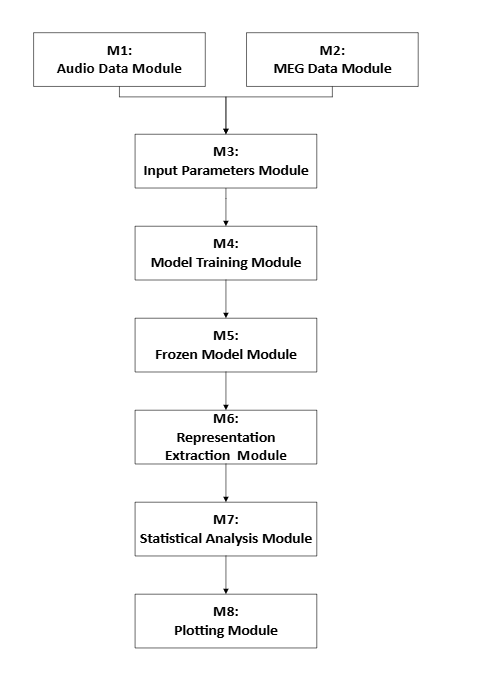
\includegraphics[width=0.7\textwidth]{framework.png}
\caption{Use hierarchy among modules}
\label{FigUH}
\end{figure}

%\section*{References}

\section{User Interfaces}

% \wss{Design of user interface for software and hardware.  Attach an appendix if
% needed. Drawings, Sketches, Figma}

The primary user interface of \progname{} is a script-based or command-line
scientific workflow. Users provide configuration parameters, dataset locations,
and model and analysis settings through files or command-line arguments. The
main user-visible outputs are analysis summaries, score tables, and saved
figures. No dedicated graphical user interface is required.






\section{Design of Communication Protocols}

% \wss{If there is communication between hardware and software, it may be necessary 
% to explain the design of the communication protocol.  This section should be filled 
% in with NA if it is not appropriate for a given project.}

N/A. \progname{} does not require a communication protocol beyond local file
access and standard operating-system services.



\section{Database Design}

% \wss{If a database is a significant component of the project, the database
% design should be summarized here.  This section should be filled in with NA if
% it is not appropriate for a given project.}

NA


\section{Timeline}

% \wss{Schedule of tasks and who is responsible}

The development schedule and division of responsibilities will be maintained in the project repository or shared project planning documents. This section may be updated later with milestones for data preparation, model training,
representation extraction, statistical analysis, and report generation.
See Github Project: \url{https://github.com/Krozix-2026/cas741-speech-trf}

% \wss{You can point to GitHub if this information is included there}

\bibliographystyle {plainnat}
\bibliography{../../../refs/References}

\newpage{}

\end{document}